% Define document class
\documentclass[twocolumn]{aastex631}
\usepackage{showyourwork}
\usepackage{tikz}
\usepackage{amsmath}
\usepackage{bm}

\usetikzlibrary{angles,patterns,calc,quotes}

% Begin!
\begin{document}

% Title
\title{Astrophysical Fluids Numerical Project}

% Author list
\author{Ted Johnson}


% Main body with filler text
\section{Oblique Shocks}
\label{sec:intro}
\begin{figure}
    \centering
    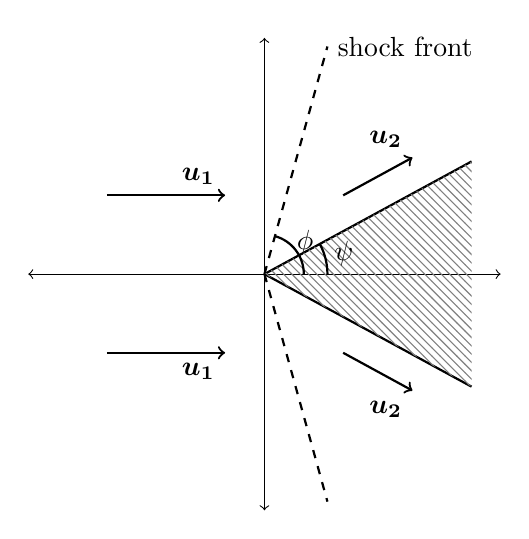
\begin{tikzpicture}
        \coordinate (O) at (0,0);
        \coordinate (xhat) at (3,0);
        \coordinate (nxhat) at (-3,0);
        \coordinate (yhat) at (0,3);
        \coordinate (nyhat) at (0,-3);
        \coordinate (u2hat) at (2.63,1.43);
        \coordinate (mu2hat) at (2.63,-1.43);
        \coordinate (corner) at (2.63,0);
        \coordinate (shock) at (0.80,2.89);
        \coordinate (mshock) at (0.80,-2.89);

        
        \draw[<->] (nxhat)--(xhat);
        \draw[<->] (nyhat)--(yhat);
        \draw[thick] (O)--(u2hat);
        \draw[thick] (O)--(mu2hat);
        \draw[thick,dashed] (O)--(shock) node[anchor=west]{shock front};
        \draw[thick,dashed] (O)--(mshock);
        \fill[pattern = north west lines, pattern color=gray] ($(O)$)--($(mu2hat)$)--($(u2hat)$);
        \pic [-,draw,angle radius=0.8cm, thick,"$\psi$",angle eccentricity=1.3] {angle = xhat--O--u2hat};
        \pic [-,draw, angle radius=0.5cm,thick,"$\phi$",angle eccentricity=1.3] {angle = xhat--O--shock};

        \draw[->, thick] (1,1)--(1.88,1.48) node[anchor=south east]{$\bm{u_2}$};
        \draw[->, thick] (1,-1)--(1.88,-1.48) node[anchor=north east]{$\bm{u_2}$};
        \draw[->, thick] (-2,1)--(-0.5,1) node[anchor=south east]{$\bm{u_1}$};
        \draw[->, thick] (-2,-1)--(-0.5,-1) node[anchor=north east]{$\bm{u_1}$};;

    \end{tikzpicture}
    \caption{Oblique shock setup. A fluid traveling at supersonic velocity $\bm{u_1}$ meets a stationary barrier of opening angle $\psi$. A shock front of opening angle $\phi$ is formed, and the post-shock fluid flows parallel to the barrier's surface at a velocity $\bm{u_2}$. Other relevant quantities to the problem include the sound speed in the pre-shock medium ($a_1$) and the adiabatic index $\gamma$.}
    \label{fig:setup}
\end{figure}
In this work we will investigate oblique shocks -- sharp discontinuities in the properties of a fluid caused by supersonic flow interacting with a barrier whose surface is not normal to the flow. Relevant quantities in this problem include the velocity of the pre-shock flow ($\bm{u_1}$), the velocity of the post-shock flow ($\bm{u_2}$), the angle between $\bm{u_1}$ and $\bm{u_2}$ ($\psi$), the angle between $\bm{u_1}$ and the normal vector to the shock $\phi$, the pre-shock sound speed $a_1$, and the adiabatic index of the gas ($\gamma$).

In the case were the angle of the shock surface ($\phi$) is not known in advance, we must deduce it from some other geometric conditions. Consider a shock caused by a wedge of known opening angle $\psi$. This setup is shown in Figure \ref{fig:setup}.

\citet{shu} gives two equations that relate these quantities:
\begin{align*}
    u_1 \cos\phi = u_2 \cos\phi \cos\psi + u_2 \sin\phi \cos\psi \, , \tag{16.17}\\
    \frac{u_2}{u_1}\cos\psi - \frac{u_2}{u_1}\cot\phi\sin\psi = \frac{2 a_1^2}{(\gamma + 1) u_1^2 \sin^2\phi} + \frac{\gamma -1}{\gamma + 1}\, . \tag{16.18}\\
\end{align*}

We can define the following dimensionless quantities to make these equations more manageable for our eventual numerical scheme:
\begin{align}
    \eta \equiv \frac{u_2}{u_1}\, , \\
    M_1 \equiv \frac{u_1}{a_1}\, .
\end{align}

And equations (16.17) \& (16.18) become
\begin{align}
    \cos\phi = \eta\cos\phi\cos\psi + \eta\sin\phi\sin\psi\, , \label{eq:eta17} \\
    \eta\cos\psi - \eta\cot\phi\sin\psi = \frac{2}{(\gamma + 1)M_1^2 \sin^2\phi} + \frac{\gamma-1}{\gamma + 1}\, . \label{eq:eta18}
\end{align}

Following the work of \citet[Ch. 16]{shu}, we can rearrange equation (\ref{eq:eta17}) to find
\begin{align}
    \tan\phi = \frac{1-\eta\cos\psi}{\eta\sin\psi}\, , \label{eq:tanphi}\\
    \sin^2\phi = \frac{(1-\eta\cos\psi)^2}{(1-\eta\cos\psi)^2+\eta^2\sin^2\psi}\, , \label{eq:sinsqphi}
\end{align}
where the second equation is found via a trigonometric relation.

\section{The Shock Polar}
We can use equations (\ref{eq:tanphi}) \& (\ref{eq:sinsqphi}) to remove $\phi$ from equation (\ref{eq:eta18}) and find that
\begin{equation}
    \label{eq:shock-polar}
    \eta^2\sin^2\psi = (1-\eta\cos\psi)^2 \frac{M_1^2\eta\cos\psi - \alpha^2}{\alpha^2 + [2/(\gamma + 1)]M_1^2 - M_1^2\eta\cos\psi}\, ,
\end{equation}
where
\begin{equation}
    \alpha^2 \equiv \frac{\gamma - 1}{\gamma + 1} M_1^2 + \frac{2}{\gamma+1}
\end{equation}
is the dimensionless critical speed. This is equivalent to $\alpha^2\equiv c_*^2/a_1^2$ in Shu's variables. Equation (\ref{eq:shock-polar}) is the {\em shock polar}, given by Shu in eq. (16.21). Solutions to this equation are shown in Figure \ref{fig:shock-polar}. See the figure caption for a discussion on the number of solutions for a given $\psi$. The extrema of $\eta$ are its two zeros: a maximum of 1, and a minimum of $\alpha^2/M_1^2$.

\begin{figure}
    \includegraphics[width=0.5\textwidth]{figures/shock_polar.pdf}
    \caption{The shock polar for various Mach numbers. For a given $\psi$ there are either two, one, or zero possible values of $\eta\equiv u_2/u_1$. When $\psi$ is small, there are two solutions possible. The one closest to the origin is called a strong shock, as the fluid becomes subsonic after the shock. The second solution is called a weak shock, as the magnitudes of the discontinuities are less, and the post-shock flow remains supersonic. For any given $M_1$, there exists a value of $\psi=\psi_\text{max}$ for which there is only one solution and the post-shock Mach number is 1 -- this represented by the dashed line for the case $M_1 \rightarrow \infty$, and by the dotted line for the case of general $M_1$. When $\psi>\psi_\text{max}$ there are no oblique shock solutions and a bow shock is formed.}
    \script{shock_polar.py}
    \label{fig:shock-polar}
\end{figure}

\subsection{Finding $\psi_\text{max}$}
For any given Mach number it is possible to find the maximum allowed deflection angle $\psi_\text{max}$ that still leads to an attached shock. It can be seen by inspection of Figure \ref{fig:shock-polar} that this angle satisfies
\begin{equation}
    \frac{d (\eta\sin\psi_\text{max})}{d (\eta\cos\psi_\text{max})} = \tan{\psi_\text{max}}\, .\label{eq:psimax_cond}
\end{equation}
The derivative on the left-hand side of equation (\ref{eq:psimax_cond}) can be computed analytically from equation (\ref{eq:shock-polar}). However, it is much easier to compute the derivative numerically using the central difference method. If we let $x\equiv\eta\cos\psi$ and $y\equiv\eta\sin\psi$, then this problem reduces to finding the solution to
\begin{equation}
    \frac{y(x+\delta)-y(x-\delta)}{2\delta} - \frac{y(x)}{x} = 0\, ,\label{eq:to_solve}
\end{equation}
for some $\delta \ll x$. For a solution $x=x_0$, we can then calculate
\begin{equation}
    \psi_\text{max} = \arctan{y_0/x_0}\, .
\end{equation}

Because there is only a single solution to equation (\ref{eq:to_solve}) and $x$ is bounded such that $\alpha^2/M_1^2 < x < 1$, we use the bisection method to find $x_0$. The dotted line in Figure \ref{fig:shock-polar} shows the position of $(x_0,y_0)$ for general $M_1$. This line separates the strong and weak shock regimes.

\section{Finding $\phi$ \& $\eta$}
In general there are two unknowns in the oblique shock problem: $\eta$ and $\phi$. Equation (\ref{eq:tanphi}) shows how $\phi$ can be easily computed once $\eta$ is known. To compute $\eta$, however, we need to use a numerical solver. We use the bisection method to solve equation (\ref{eq:shock-polar}). We choose this solver again because of its simplicity and stability.

In order to find the value of $\eta$ for both a strong and weak shock we run our solver twice over two different domains:
\begin{eqnarray}
    \alpha^2/M_1^2 <\,& \eta_\text{strong}\cos\psi &< \eta_{\psi_\text{max}}\cos\psi_\text{max}\,  ,\\
    \eta_{\psi_\text{max}}\cos\psi_\text{max} <\,& \eta_\text{weak}\cos\psi &< 1\, .
\end{eqnarray}

The bisection method allows this domain to be strictly enforced, while other methods (e.g. Newton-Raphson) are susceptible to large jumps which can lead to unexpectedly finding a solution other than that which is intended.

Now that $\eta$ can be found for any (attached shock) setup in both the strong and weak regimes, we solve for $\psi$ using equation (\ref{eq:tanphi}). Figure \ref{fig:phi} shows the results in both the strong and weak regimes using the parameterization $\phi = \phi(\psi;M_1,\gamma)$.


\begin{figure}[t]
    \includegraphics[width=0.5\textwidth]{figures/phi.pdf}
    \caption{Shock angle solutions. The transition between strong (lower portion) and weak (upper portion) occurs and the $\psi$-maximum of each curve. This transition is marked by the dotted line.}
    \script{phi.py}
    \label{fig:phi}
\end{figure}

Strong and weak shock solutions for $\phi$ are shown in Figure \ref{fig:phi}.

\section{Discussion}


\bibliography{bib}

\end{document}
